\documentclass[tikz,border=3pt]{standalone}
\usepackage[utf8]{inputenc}
\usepackage[T1]{fontenc}
\usepackage{lmodern}
\renewcommand{\familydefault}{\sfdefault}
\usepackage{sansmath}\sansmath
\usepackage{chemfig}
\usepackage{pgfplots}\pgfplotsset{compat=1.18,/pgf/number format/use comma,/pgf/number format/1000 sep={.}}
\usetikzlibrary{arrows.meta,calc,positioning,decorations.pathmorphing,patterns}
% paleta del sitio
\definecolor{nar}{HTML}{E8680C}\definecolor{narc}{HTML}{FFB35C}\definecolor{hielo}{HTML}{FFF3E8}
\definecolor{tinta}{HTML}{1D1D1F}\definecolor{gris}{HTML}{6E6E73}\definecolor{lila}{HTML}{7C5CF0}
\definecolor{azul}{HTML}{2F6FD6}\definecolor{menta}{HTML}{17A673}\definecolor{coral}{HTML}{E8342A}
\begin{document}
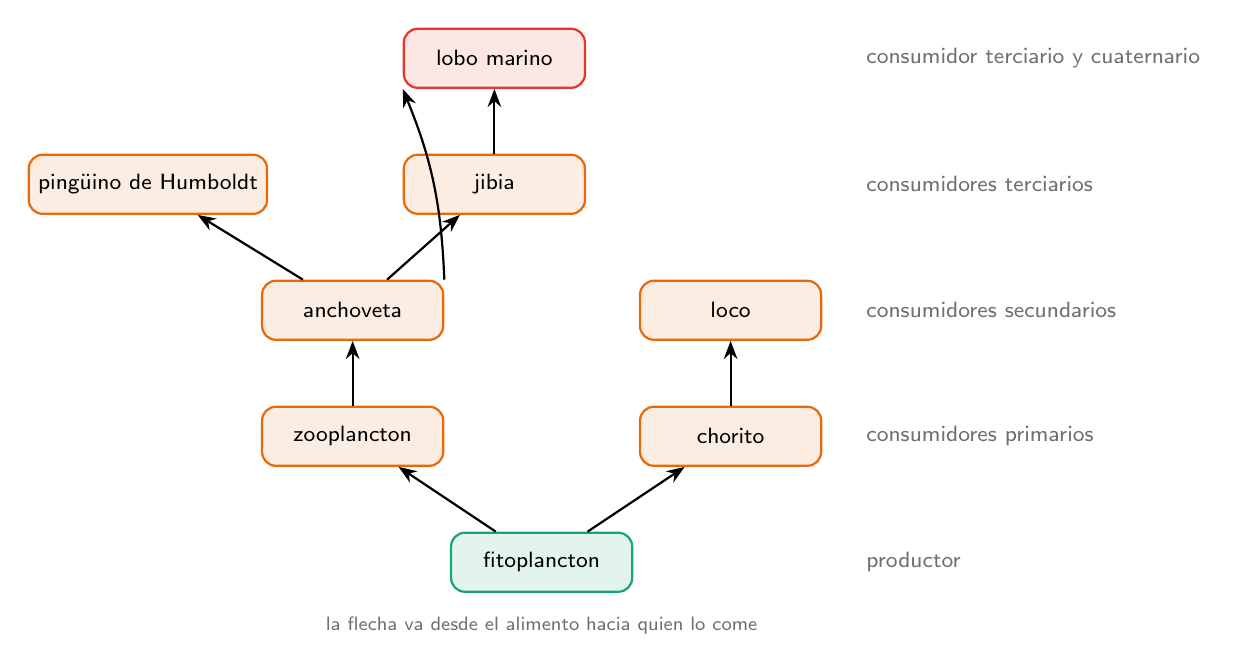
\begin{tikzpicture}[font=\footnotesize,>={Stealth[length=2.3mm]}]
\tikzset{esp/.style={draw=#1,fill=#1!12,thick,rounded corners=5pt,minimum width=2.3cm,minimum height=0.75cm,align=center}}
\node[esp=menta] (fit) at (3.6,0) {fitoplancton};
\node[esp=nar] (zoo) at (1.2,1.6) {zooplancton};
\node[esp=nar] (cho) at (6.0,1.6) {chorito};
\node[esp=nar] (anc) at (1.2,3.2) {anchoveta};
\node[esp=nar] (loc) at (6.0,3.2) {loco};
\node[esp=nar] (pin) at (-1.4,4.8) {pingüino de Humboldt};
\node[esp=nar] (jib) at (3.0,4.8) {jibia};
\node[esp=coral] (lob) at (3.0,6.4) {lobo marino};
\draw[->,thick] (fit) -- (zoo); \draw[->,thick] (fit) -- (cho);
\draw[->,thick] (zoo) -- (anc); \draw[->,thick] (cho) -- (loc);
\draw[->,thick] (anc) -- (pin); \draw[->,thick] (anc) -- (jib);
\draw[->,thick] (jib) -- (lob); \draw[->,thick] (anc.north east) to[bend right=10] (lob.south west);
\node[anchor=west,text=gris,align=left] at (7.6,0) {productor};
\node[anchor=west,text=gris,align=left] at (7.6,1.6) {consumidores primarios};
\node[anchor=west,text=gris,align=left] at (7.6,3.2) {consumidores secundarios};
\node[anchor=west,text=gris,align=left] at (7.6,4.8) {consumidores terciarios};
\node[anchor=west,text=gris,align=left] at (7.6,6.4) {consumidor terciario y cuaternario};
\node[text=gris,font=\scriptsize] at (3.6,-0.8) {la flecha va desde el alimento hacia quien lo come};
\end{tikzpicture}
\end{document}
